%%%%%%%%%%%%%%%%%%%%%%%%%%%%%%%%%%%%%%%%%%%%%%%%%%%%%%%%%%%%%%%%%%%%%
% AGUJournalTemplate.tex

%% To submit your paper:
\documentclass[draft,linenumbers,onecolumn]{agujournal2019} % set options to [final] after final review
\usepackage{array}
\newcolumntype{P}[1]{>{\centering\arraybackslash}m{#1}}
\usepackage{url} %this package should fix any errors with URLs in refs.
\usepackage[inline]{trackchanges} %for better track changes. final option will compile document with changes incorporated.
\usepackage{soul}
\usepackage{multirow}
\usepackage{amsmath}
\usepackage{float}
\usepackage{placeins}
\usepackage{float}
%%%%%%%
% As of 2018 we recommend use of the TrackChanges package to mark revisions.
% The trackchanges package adds five new LaTeX commands:
%
%  \note[editor]{The note}
%  \annote[editor]{Text to annotate}{The note}
%  \add[editor]{Text to add}
%  \remove[editor]{Text to remove}
%  \change[editor]{Text to remove}{Text to add}
%
% complete documentation is here: http://trackchanges.sourceforge.net/
%%%%%%%

% specific packages (added by Sebastian)
\usepackage{bm}
\usepackage{amssymb}

\journalname{Water Resources Research}

\begin{document}

\title{Multi-output Gaussian process optimizes roughness parameters for morphological units in 2d numerical models}

\graphicspath{ {./images/} }

%% ------------------------------------------------------------- %%
%
%  AUTHORS AND AFFILIATIONS
%
%% ------------------------------------------------------------- %%

\authors{Andres Heredia \affil{1}, Sebastian Schwindt\affil{1}, Silke Wieprecht\affil{1}, Sergey Oladyshkin\affil{2}}

\affiliation{1}{Institute for Modelling Hydraulic and Environmental Systems,
	Department of Hydraulic Engineering and Water Resources Management, University of Stuttgart, Stuttgart, Germany}

\affiliation{2}{Institute for Modelling Hydraulic and Environmental Systems, 
	Department of Stochastic Simulation and Safety Research for Hydrosystems, SC SimTech, University of Stuttgart, Stuttgart, Germany}


%% Corresponding Author:
% Corresponding author mailing address and e-mail address:
\correspondingauthor{Andres Heredia}{andres.heredia-hidalgo@iws.uni-stuttgart.de}

%% Keypoints, final entry on title page.
\begin{itemize}
	\item Surrogate-assisted calibration for 2d hydro-morphodynamic models using multi-output Gaussian process regression and Bayesian active learning.
	\item Uncertainty quantification of riverbed surface roughness for selected morphological units around large wood pieces.
	\item Comparison between single-output and multi-output Gaussian process outcomes  \hl{SHOWS ... - PUT KEY FINDING}.
\end{itemize}

%% --------------------------------------------------------------- %%
%
%  ABSTRACT and PLAIN LANGUAGE SUMMARY
%
%% --------------------------------------------------------------- %%

%% \begin{abstract} starts the second page

% --- AUTHORS CLAP OUT THE COMMENT BAR --- --- --- --->>>

\begin{abstract}
% max. 250 words (curr. 249) -- A NEW WORD REQUIRES DELETION
	
	
\textit{KEYWORDS: Multitask Gaussian process regression, Bayesian active learning, Telemac2d, metamodels, hydro-morphodynamic modeling}
\end{abstract}

\section*{Plain Language Summary}
% currently 196/200 words, accounting for AGU recommendations (https://www.agu.org~s\textsuperscript{-1}hare-and-Advocate~s\textsuperscript{-1}hare/Community/Plain-language-summary)
\hl{do not use technical terms like Gaussian, metamodel, correlate, roughness etc.}

The real behavior of rivers can be simulated using conceptual computer models. These models are often highly complex and computationally demanding because they must represent detailed, coupled physical processes such as water and sediment dynamics, requiring the introduction of several uncertain model parameters and hindering the identification of plausible parameter combinations which lead to acceptable resemblance to reality. To alleviate this, we use a multi-output machine learning approach to approximate model responses (i.e., water depth and scalar velocity) from a highly complex hydromorphodynamic model. This method helps perform data-driven stochastic calibration and uncertainty quantification of model parameters that lead to a desired and plausible resemblance of the model to measured velocity and water depth. We find that...   


\section{Introduction}

River restoration employs a variety of measures, including the artificial creation of distinct morphological patterns, the large wood placement, and vegetation plantings  \cite{schwindt2019hydromorphological, kail2007usea, roni2015wood, grabowski2019current, neuhaus2021engineered}. These interventions modify hydro-morphodynamic processes and change or are compromised by strong currents, particularly during floods and associated topographic changes. Numerical simulations offer critical insight into assessing the longevity of restoration measures and their effectiveness in attenuating flood waves and improving habitat quality \cite{schwindt2020river}. Nevertheless, even high-resolution two-dimensional (2d) and three-dimensional (3d) models often suffer from considerable uncertainties and inaccuracies that stem from numerous simplifying assumptions. For instance, wall roughness generates internal friction and thus turbulence, which substantially influences the momentum balance in numerical models. Owing to the complexity of river landscapes, detailed representation of wall-roughness effects is frequently replaced by bulk roughness models, such as Manning's~$n$ \cite{manning1891flow} or the Strickler roughness coefficient \cite{strickler1923beitrage, meyer-peter1948formulas}. Using these bulk parameters can blur the distinction between grain-scale and morphological-unit-scale roughness \cite{ferguson2007flow}, which is difficult to resolve during model calibration, especially when the computational mesh is too coarse to depict individual morphological units. Clear differentiation among morphological units is therefore essential, and the mesh resolution must be fine enough to represent them explicitly.

Large wood (LW) has been shown to be an efficient restoration measure that enhances habitat quality by generating advantageous hydraulic flow patterns \cite{follett2020momentum, schalko2024enhanced} and by improving sedimentary conditions, particularly grain-size composition and oxygenation \cite{schwindt2023fuzzylogic, schalko2024flow}. These insights are based solely on field surveys and laboratory flume experiments because numerical simulations of sediment-related processes remain highly uncertain. In particular, simulating riverbed clogging, defined as the infiltration of fine sediment into the pore space of a coarser sediment matrix, remains challenging. Clogging impairs aquatic habitats by cutting off vertical exchange, which reduces oxygen availability and increases substrate compactness, thus degrading spawning grounds and ecological niches of macroinvertebrates and microorganisms \cite{banscher1976gesetzmassigkeiten, brunke1997ecological, blaschke2003clogging}. Accurate modeling of clogging requires simultaneous simulation of subsurface and surface hydrodynamics, including advective and diffusive particle transport. State-of-the-art modeling approaches cannot yet perform these coupled simulations for the hydraulically distinct zones beneath and above the bed. Yet, the accumulation of fine sediment within the substrate can already be estimated reliably with coupled hydrodynamic-morphodynamic 2d models \cite{scolari2025hydromorphodynamic}.

Artificial intelligence offers a promising pathway to improve the calibration of numerical models. For instance, supervised learning that combines Bayesian inference with metamodels (also called surrogate models) allows evaluation of a wide range of calibration-parameter combinations. Bayesian active learning (BAL) constructs a probabilistic surrogate, typically a Gaussian process, that represents the misfit between the output of a deterministic numerical model and observed data, using results from prior simulations. In BAL, the long computing time of the numerical model is often replaced by a Gaussian process emulator (GPE) that approximates the response surface of the complex numerical model. After each computationally expensive numerical model run, BAL updates the surrogate and applies an acquisition function to choose the next parameter set, balancing exploitation of the current optimum against exploration of uncertain regions. This strategy yields well-calibrated parameters with fewer simulations than heuristic optimum searches \cite{oladyshkin2020bayesian3,rasmussen2006gaussian}. 

Calibration with BAL starts with a set of numerical model runs (typically 15 per calibration parameter) to explore model responses across a parameter range in which each value is initially (\textit{a priori}) assumed to be equally likely. As information accumulates, the probability distribution is updated until either BME or relative entropy (RE, also referred to as Kullback-Leibler divergence, cf. \citeA{kullback1951informationa}) converges. Consequently, each calibration parameter is assigned a nonuniform, typically Gaussian-distributed, \textit{a posteriori} probability density function. The peak of this function marks the statistically best-fitting value, and the width of the distribution quantifies the remaining uncertainty. A broad distribution indicates high uncertainty, while a narrow one indicates low uncertainty \cite{oladyshkin2020bayesian3}. This approach has already been shown to be highly efficient for optimizing simulations of hydro-morphodynamic processes in rivers \cite{beckers2020bayesian}, and it has exposed physical inconsistencies in simulations of reservoir sedimentation \cite{mouris2023stability}. However, BAL can also lead to overfitting, although calibrating multiple parameters simultaneously flags when this occurs. Overfitting, or equifinality, especially arises when the available measurement data are insufficient to describe the target phenomena. For instance, if background eddy viscosity and diffusivity are treated as calibration parameters but flow velocity is not supplied to the BAL calibration, the resulting \textit{a posteriori} distributions exhibit high uncertainty \cite{schwindt2023bayesian}.

The simultaneous calibration of multiple parameters is challenging not only for heuristic methods but also for advanced techniques such as BAL. The BAL algorithms currently available for optimizing hydro-morphodynamic surface-water models perform only sequential calibration of multiple parameters \cite{mouris2023stability,schwindt2023bayesian}. A sequential approach, however, prevents iterative and simultaneous consideration of parameter interactions and cannot accommodate spatially explicit parameter values, such as zonal roughness coefficients assigned to distinct morphological units. To overcome these limitations, this study applies multi-output learning with Gaussian processes, which permits the full incorporation of coupled physical processes that cannot be treated in isolation \cite{bonilla2007multitask}. Accordingly, this study addresses the following research question: \textit{How does BAL employing multi-output GPE compare with BAL using single-output GPE in terms of statistical and physical performance when different roughness zones are defined for distinct morphological flow patches upstream and downstream of large-wood placements?}

To answer this question, this study extends existing BAL algorithms by incorporating a multi-output Gaussian-process emulator (MO-GPE). A 215 m long 2d hydro-morphodynamic numerical model of a near-natural fishway that includes the targeted placement of two LW pieces was built with distinct roughness zones for apparent morphological units (MUs) of the main channel. The numerical model was developed and BAL-calibrated with data from earlier studies \cite{schwindt2023fuzzylogic, schalko2024flow, scolari2025hydromorphodynamic}. The null hypothesis (H0) is that, when calibrating spatially explicit roughness zones upstream and downstream of LW placements, BAL with MO-GPE achieves better statistical performance as BAL with single-output Gaussian-process emulators (SO-GPE), as measured by the \hl{root-mean-squared error for water depth and depth-averaged flow velocity}. Under H0, the spatial patterns of water depth, and depth-averaged flow velocity predicted by BAL with MO-GPE are more similar to field observations than those predicted by SO-GPE, as evaluated with the spatial Spearman rank correlation upon the convergence of Kullback-Leibler divergence (i.e., RE) and  Bayesian Model Evidence (i.e., BME). The alternative hypothesis (H1) is that, under the same calibration scenario, BAL with MO-GPE yields median \hl{at least a 10\% reduction in RMSE} for the same variables, and produces spatial Shields stress, water depth, and flow velocity patterns with a \hl{Spearman} correlation at least 0.10 lower and a Kullback-Leibler divergence \hl{or BME?} at least 10\% higher than those obtained with SO-GPE.


\section{Materials and Methods} 
\label{sec:methods}

\subsection{Testbed: Morphodynamic Fishway}
\label{sec:testbed}

This study was carried out at the Ering-Frauenstein hydropower plant, where a 2.6 km-long fishway with a 5--10 m-wide gravel-bed bypasses the dam and surmounts a 10~m head at an average longitudinal bed slope of 4.7\textperthousand \cite{zauner2020wie}. Gravel that flows through the fishway collects in a sediment trap at the downstream end. This sediment is then transported to the upstream end mannually to enable morphodynamic development during artificial morphologically effective floods conducted each year.

In this study, a 215 m-long reach served as the domain for the numerical model. In this reach, two LW pieces were installed perpendicular to the flow to investigate riverbed clogging in  January 2022. An artificial flood was then generated by raising discharge from the 2~m\textsuperscript{3}~s\textsuperscript{-1} baseflow to 9.7~m\textsuperscript{3}~s\textsuperscript{~1} via an inlet weir. The two LW pieces, referred to as log~A (363 071.83, 5 350 214.56) and log~B (363 118.99, 5 350 254.67) in UTM Zone 33N (see \ref{fig:study-area}), were found to reduce clogging under specific flow conditions \cite{schwindt2023fuzzylogic,schalko2021flow,schalko2024flow}. These conditions were partly reproduced with a 2d hydro-morphodynamic Telemac2d/Gaia model \cite{scolari2025hydromorphodynamic}.



\begin{figure}[htbp]
	\centering
	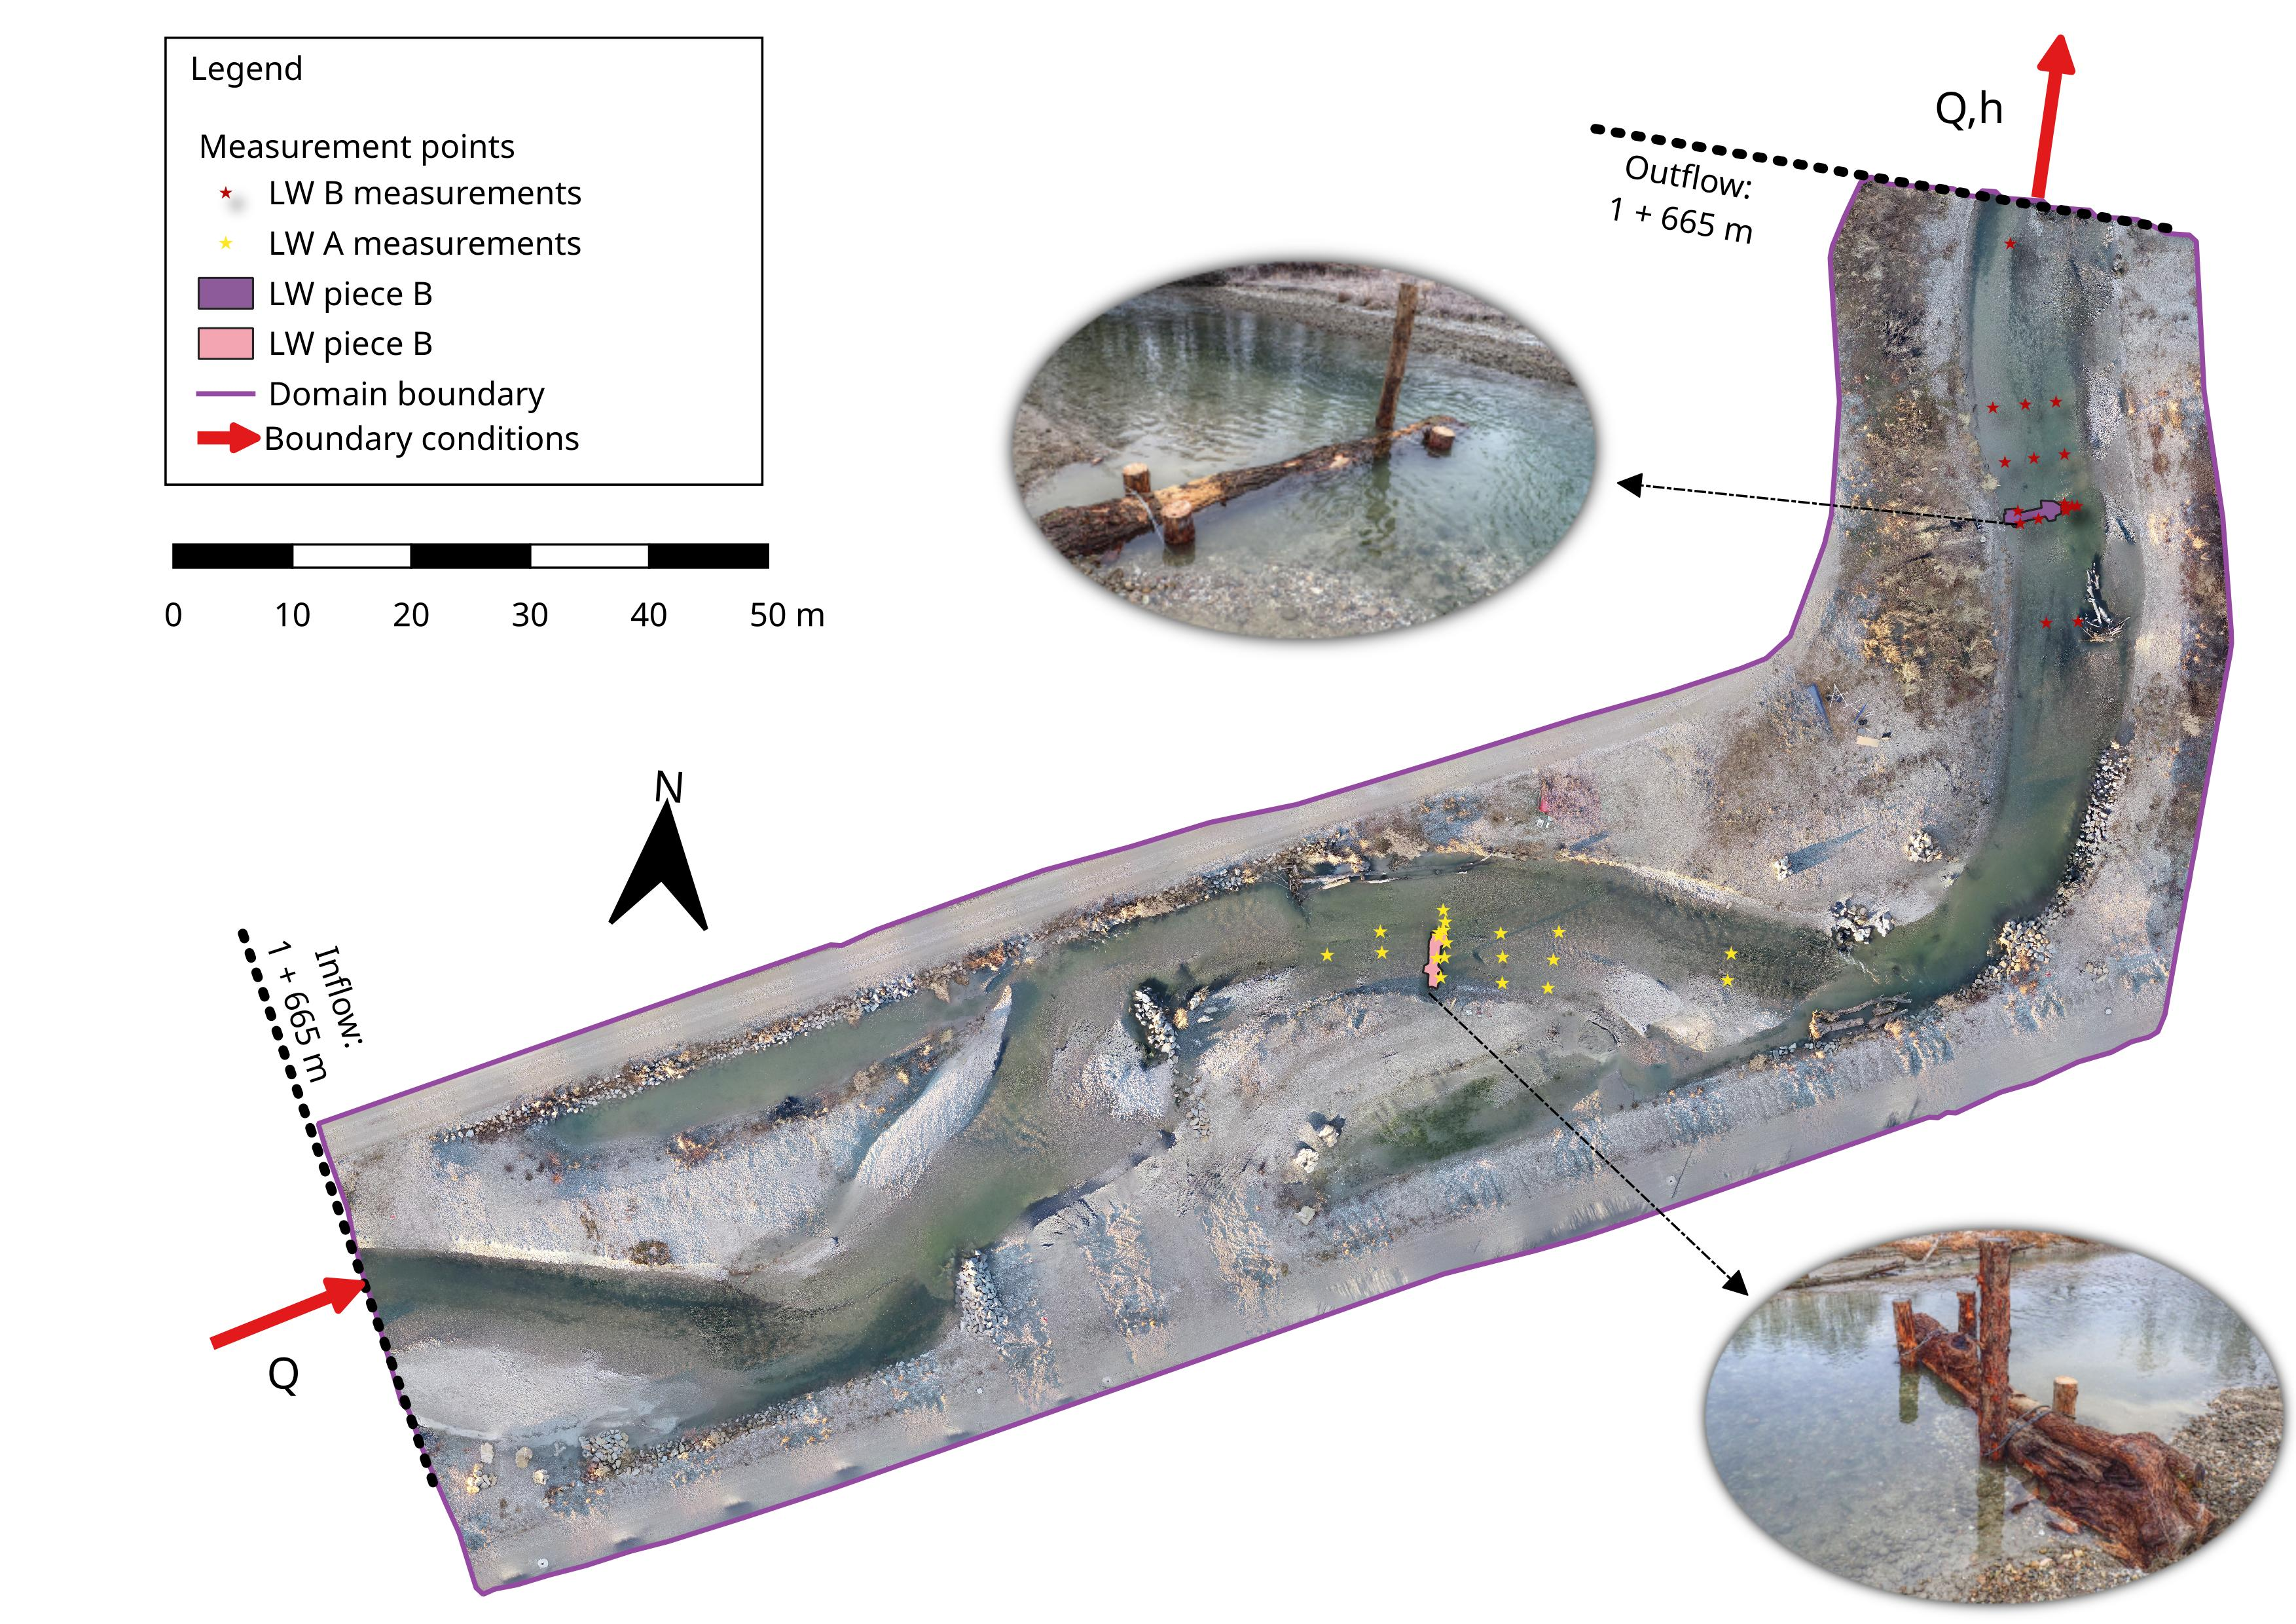
\includegraphics[width=0.99\textwidth]{1_study-area.jpg}
	\caption{The considered reach at the fishway, including the two LW pieces, log~A (upstream) and log~B (downstream).	}
	\label{fig:study-area}
\end{figure}

The locations of available measurement data in addition to MUs are shown in Figure~\ref{fig:study-area}. Discharge was recorded using a boat-mounted acoustic Doppler current profiler (ADCP) at two cross-section that are not indicated in Figure~\ref{fig:MU}, and during the artificial flood. The inflow hydrograph is plotted in Figure ~\ref{fig:inflow-hydrograph}.

\begin{figure}[htbp]
	\centering
	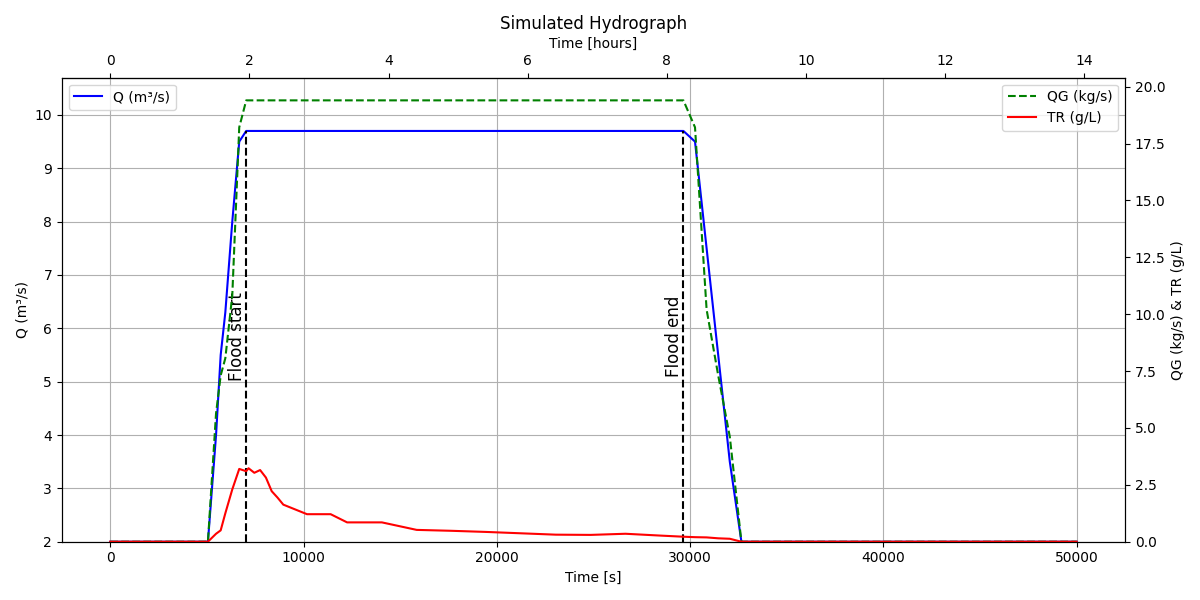
\includegraphics[width=0.99\textwidth]{2_hydrograph.png}
	\caption{Simulated liquid and solid influx.	}
	\label{fig:inflow-hydrograph}
\end{figure}
Hydraulic data, including flow velocity and water depth, was collected at 37 positions in the considered reach with a FlowTracker2 (acoustic Doppler velocimeter, ADV) device under baseflow conditions after the artificial flood. The 37 points corresponded to locations where the hydro-morphodynamic footprint of the LW pieces was assumed to be significant, in addition to representative MUs, including pools, slackwater, glides, riffles, and runs. The MUs were delineated according to criteria summarized in \citeA{montgomery1997channelreach} and \citeA{wyrick2014geospatial} (\hl{see detaild in the SI}). Digital elevation models (DEMs) with a resolution of 0.05 m were created using UAS RGB orthoimagery. The grain size characteristics of the subsurface (hyporheic zone) and surface (riverbed) sediment layers, listed in Table~\ref{tab:grain-sizes}, were quantified using frozen sediment cores and shovel samples, respectively, under below-baseflow conditions (0.5~m\textsuperscript{3}~s.\textsuperscript{-1}) (see \citeA{schwindt2023fuzzylogic, negreiros2024database, scolari2025hydromorphodynamic}).

\begin{table}[h]
	\centering
	\caption{Grain size characteristics of the subsurface (hyporheic zone) and surface (riverbed) substrate layers (sources: \citeA{negreiros2024database, scolari2025hydromorphodynamic}).}
	\begin{tabular}{lcccccccc}
		\hline
		\textbf{Percentile} & $d_{10}$ & $d_{16}$ & $d_{30}$ & $d_{50}$ & $d_{60}$ & $d_{84}$ & $d_{90}$ & $d_m$\\
		Subsurface (mm)       & 0.14 & 0.21 & 1.11 & 10.36 & 15.08 & 37.17 & 48.30 & 17.76 \\
		Surface (mm)          & 0.39 & 1.27 & 6.25 & 14.92 & 22.25 & 48.25 & 56.19 & 23.79 \\
		\hline
	\end{tabular}
	\label{tab:grain-sizes}
\end{table}

\subsection{Numerical model setup}
\label{sec:numerical-model}

%Descripction of Telemac2d and Gaia, bed transport equation
A 2d hydro-morphodynamic model of the 215~m-long section was created in Telemac2d \cite{hervouet2020telemac2d} along with its sediment transport and topographic change module Gaia \cite{tassi2023gaia}. Telemac2d is a  versatile open-source software that iteratively solves the depth-averaged shallow water equations \cite{saint-venant1871theorie} over an unstructured mesh through either finite element or finite volume methods \cite{galland1991telemac,hervouet2007hydrodynamics}. It is indirectly coupled with the Gaia module that computes sediment transport and topographic change.  Topographic change is computed by solving the Exner equation at each computational timestep \cite{exner1925uber,audouin2020introducing}. It accounts for the spatial and temporal variability of sediment characteristics, including multiple sediment size classes stored in an active surface layer and subsurface layers \cite{hirano1971riverbed}. 

In this study, bedload was modeled in Gaia with the Meyer-Peter Müller formula \cite{meyer-peter1948formulas} and the Wong-Parker correction \cite{wong2006reanalysis} using five sediment classes representing the characteristic grain sizes shown in Table~\ref{tab:grain-sizes}. Each class was assigned a critical Shields parameter \cite{shields1936anwendung} value for incipient motion. The two substrate layers were 0.08~m (surface) and a 0.6~m (subsurface) thick \cite{scolari2025hydromorphodynamic}. The solid influx accounts for bedload estimated with the Meyer-Peter \& Müller formula at the inlet and suspended load concentrations, measured in g~L\textsuperscript{-1} during the artificial flood.

A triangular computational mesh with elements edge lengths of 0.5~m in the active channel, and 1~m on the floodplain discretized the computational domain spatially. Figure~\ref{fig:mu_mesh} shows the computational mesh with a total of 11,738 nodes and 22,997 elements and the assigned boundary conditions.

%\hl{COMMENTS ON 2\_EringFishpass\_mesh: (1) The downstream boundary should be denotes "prescribed Q, h" (no capital because in the manuscript water depth is h, not H). (2) Please add the roughness zones here. (3) Point with arrows on the to LW pieces. (4) This figure partially double-up information that is already visibile in Figure 1, so consider moving it to the SI.} - Done

\begin{figure}[!htbp]
	\centering
	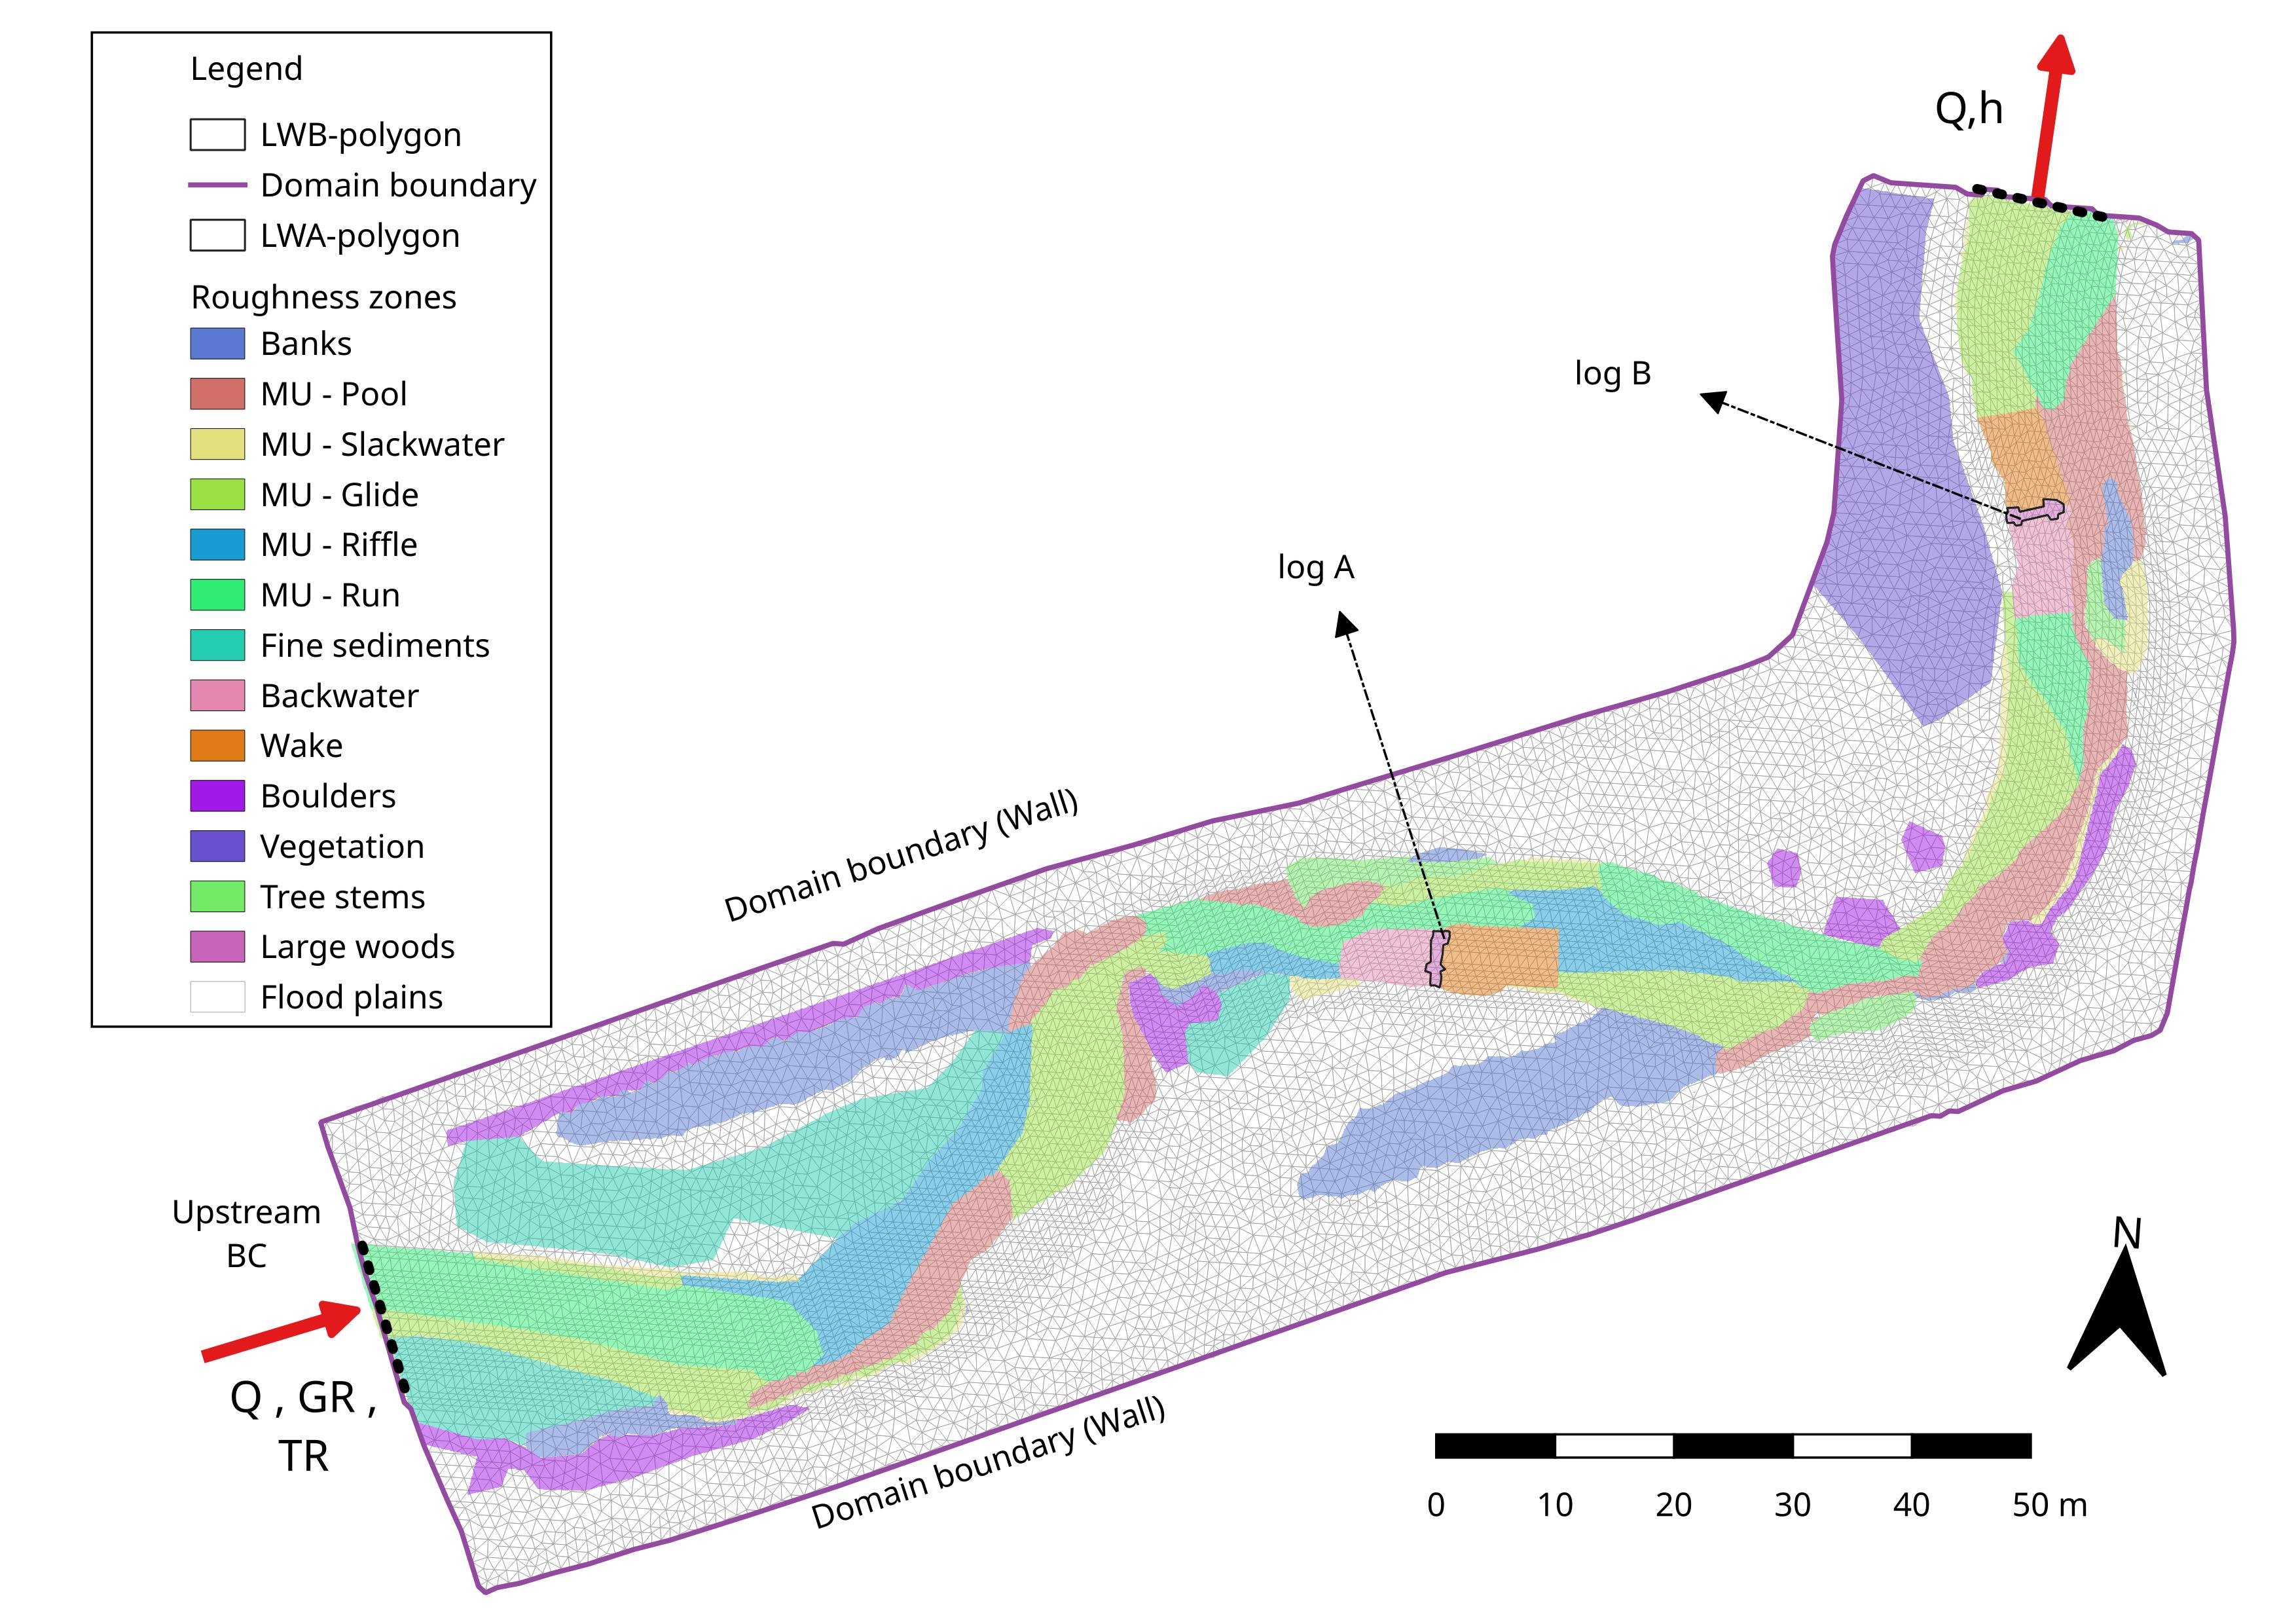
\includegraphics[width=5.5in]{3_MU+mesh.jpg}
	\caption{Mesh of the numerical model, with indication of boundaries, the two LW pieces, and roughness zones \hl{move to SI?}.}
	\label{fig:mu_mesh}
\end{figure}


% Roughness zones
The computational mesh has 14 roughness zones and among them the delineation of MUs were considered (Figure~\ref{fig:mu_mesh}). The simulation uses the Nikuradse equivalent roughness length $k_{NKU}$  \cite{nikuradse1933stroemungsgesetze} to describe the surface roughness height of the riverbed and bank. Five zones corresponded to MUs, and the remaining three zones described the backwater and wake regions as well as the wood log pieces themselves (see Table~\ref{tab:roughness-shields}). The delineation criteria of MUs are described in the \textit{Supplemental Information} file. 

%\hl{SI - PLEASE MOVE MU DELINEATION DETAILS TO THE SI}.


Each in-channel roughness zone, $k_{NKU}$ and the critical Shields parameters, which is related to the mean grain size of the surface layer (\hl{IMPORTANT -- see email}) , were considered calibration parameters. Thus, eight zonal $k_{NKU}$  and $\tau_{*,cr,m}$  were sampled from uniform distributions ($U$) with fixed bounds, as listed in Table~\ref{tab:roughness-shields}. An initial model run was performed using $k_{NKU}$~=~3$\times d_{50}$ and $\tau_{*,cr,m}$~=~0.047 to start the BAL process. 

%\hl{1 -- why did you start with 0.048 for the Shields parameter? The common sense is to start with 0.047, which is defined as the basis for everything. So I changed this in  the text above, but please also make sure to correctly implement 0.047 in your code -- starting with 0.048 cannot be defended in front of any reviewer.} - Done

%\hl{2 -- TABLE model parameters was mixing up a lot of information that had already been mentioned in the text. So I moved it to the SI.}

\begin{table}[H]
	\centering
	\caption{Roughness parameters and critical Shields parameters $\tau_{*,cr,m}$ with uniform distribution $\mathcal{U}$ bounds considered in the calibration process with BAL.}
	\begin{tabular}{
			>{\centering\arraybackslash}p{5.5cm} 
			>{\centering\arraybackslash}p{3cm} 
			>{\centering\arraybackslash}p{5.5cm}
		}
		\hline
		\textbf{Parameter} & 
		\textbf{Value} & 
		\textbf{Calibration Range} \\ \hline
		
		\multicolumn{3}{l}{\textbf{--- Roughness zones ---}} \\
		
		Banks                    & 0.050   & None \\
		Boulder                 & 1.5     & None \\
		Fine sediment           & 0.002   & None \\
		Floodplain              & 0.075   & None \\
		Tree stems              & 0.22    & None \\
		Vegetation              & 0.070   & None \\ \hline
		
		\textbf{* Glide}         & $k_{\text{glides}}$        & $\mathcal{U}(0.002, 0.6)$ \\
		\textbf{* LW}            & $k_{\text{LW}}$            & $\mathcal{U}(0.002, 2.8)$ \\
		\textbf{* LW Backwater}  & $k_{\text{backwater}}$     & $\mathcal{U}(0.002, 0.6)$ \\
		\textbf{* LW Wake}       & $k_{\text{wake}}$          & $\mathcal{U}(0.04, 0.6)$ \\
		\textbf{* Pool}          & $k_{\text{pools}}$         & $\mathcal{U}(0.008, 0.6)$ \\
		\textbf{* Riffle}        & $k_{\text{riffles}}$       & $\mathcal{U}(0.002, 0.6)$ \\
		\textbf{* Run}           & $k_{\text{runs}}$          & $\mathcal{U}(0.04, 0.6)$ \\
		\textbf{* Slackwater}    & $k_{\text{slackwater}}$    & $\mathcal{U}(0.008, 0.6)$ \\ \hline
		
		\multicolumn{3}{l}{\textbf{--- Critical Shields parameters ---}} \\
		
		\textbf{$d_{10}$}           & $\tau_{*,cr,d_{10}}$         & $\mathcal{U}(0.047, 0.070)$ \\
		\textbf{$d_{\text{mean}}$} & $\tau_{*,cr,d_{\text{mean}}}$ & $\mathcal{U}(0.047, 0.070)$ \\
		
	\end{tabular}
	\label{tab:roughness-shields}
\end{table}




\subsection{Calibration with Bayesian active learning}
\label{sec:bal}

\subsubsection{Bayesian active learning (BAL)}
\label{sec:bal-inference}

%Calibration reduces the discrepancy between model outputs and observed data by modifying sensitive input parameters \cite{oberkampf2004verification}. Bayesian calibration supports this process by accounting for sources of uncertainty in the calibration parameter space $\omega = \left{\omega_1, \omega_2, \ldots, \omega_N\right}$. Calibration in the BAL context applies Bayes' theorem to iteratively update a probabilistic surrogate (here, an SOGPE or MO-GPE) that represents the discrepancy between model output and observations. After each computationally costly numerical simulation, the posterior distribution is revised, and an acquisition function selects the next parameter set expected to yield the greatest information gain, balancing exploration of uncertain regions with exploitation of current optima \cite{rasmussen2006gaussian}. 

The prior probability functions are updated through a measurement data vector  $\mathbf{D}$ using a likelihood function~$P(\mathbf{D} | \mathbf{\Omega} , \mathcal{M}_c)$, where $P(\cdot)$ denotes a probability density function (pdf) and $\mathcal{M}_c$~denotes the deterministic (Telemac2d-Gaia) model. The likelihood function (of parameter values $\mathbf{\Omega}$) expresses how statistically likely it is to observe the data $\mathbf{D}$ if the combination of $\mathbf{\Omega},\mathcal{M}_c$ was true. In the context of Bayesian updating using a model $\mathcal{M}_c$, Bayes' theorem reads as follows \cite{oladyshkin2020bayesian3}: 

\begin{equation} \label{eq:bayes}
	P\left( \mathbf{\Omega} \vert \mathbf{D},\mathcal{M}_c \right) = \frac{P\left( \mathbf{D} \vert \mathbf{\Omega},\mathcal{M}_c \right) \cdot P\left( \mathbf{\Omega}\vert \mathcal{M}_c\right) }{P\left( \mathbf{D}\vert\mathcal{M}_c\right)}
\end{equation}

where, $P(\mathbf{\Omega} \vert \mathcal{M}_c)$ denotes the prior probability-density function of the model parameters, encapsulating expert knowledge derived from previous simulations and measurements. Combining this prior information with the calibration data transforms the prior $P(\mathbf{\Omega} \vert \mathcal{M}_c)$ into the posterior distribution $P(\mathbf{\Omega} \vert \mathbf{D}, \mathcal{M}_c)$, which is necessarily at least as informative as the prior \cite{box1973bayesian,oladyshkin2019connection}. The denominator $P(\mathbf{D} \vert \mathcal{M}_c)$, also known as Bayesian model evidence (BME), acts as a normalizing constant in Bayes' theorem, yet it is pivotal for comparing competing models and diagnosing potential model error.

The efficient application of BAL requires thousands of model~$\mathcal{M}_c$ runs to update the prior distribution, for instance, with Monte Carlo or Markov-Chain Monte Carlo methods. However, the hydro-morphodynamic numerical model can practically not run thousands of times, as this would result in years-long computing time \cite{oladyshkin2020bayesian3}. Therefore, metamodels are commonly applied for BAL-based calibration of hydro-morphodynamic models \cite{beckers2020bayesian, mouris2023stability, schwindt2023bayesian}.  A metamodel  $\mathcal{M}$ runs up to 10\textsuperscript{6} times faster than a complex numerical model  $\mathcal{M}_c$ and emulates its response surface with minimum statistical error \cite{beckers2020bayesian}.

With a fast-performing metamodel, Bayesian inference was conducted using 22,000 Monte Carlo (MC) samples to infer updated probability distributions of ten uncertain calibration model parameters (see Table ~\ref{tab:roughness-shields}) through rejection sampling \cite{smith1992bayesian}. In this approach, imperfections in the two modeling approaches (numerical and metamodels) were quantified using the measurements by considering a lump sum of uncertainties, combining measurement error, complex model error, and the additional error introduced by the metamodel approximation following a Gaussian distribution. The likelihood function of the observed data given a Monte Carlo realization vector $\omega_{\text{MC}}$ is:

\begin{equation} \label{eq:mc}
	P(\mathbf{D} \mid \omega_{\text{MC}}) = \mathcal{N}(\mathbf{D} \mid \mathcal{M}(\omega_{\text{MC}}), \bm{R})
\end{equation}

where $\mathcal{M}_c(\omega_{\text{MC}})$ is a vector containing the metamodel predictions at $P$ measurement locations and $\bm{R} \in \mathbb{R}^{P \times P}$ is the total covariance matrix over all measurement locations as

\begin{equation} \label{eq:covar}
	\mathbf{R} = \sum_{p=1}^{P} \left( \mathbf{\Sigma}_{\text{complex}} + \mathbf{\Sigma}_{\text{surrogate}} + \mathbf{\Sigma}_{\text{measurement},p} \right)
\end{equation}

Note that if the likelihood function incorporates more than one variable, it becomes a multivariate likelihood. In this study, when using the MO-GPE metamodel the likelihood employs the two metamodel outputs from the multi-output metamodel (i.e., water depth and velocity) to compute a multivariate likelihood , doubling the size of the necessary vectors and matrices for likelihood computation. The expanded likelihood function becomes: 

\begin{equation} \label{eq:}
	P(\mathbf{D} \mid \omega_{\text{MC}}) = \frac{1}{\sqrt{(2\pi)^P |\bm{R}|}} \exp\left( -\frac{1}{2} \left( \mathbf{D} - \mathcal{M}(\omega_{\text{MC}}) \right)^\top \bm{R}^{-1} \left( \mathbf{D} - \mathcal{M}(\omega_{\text{MC}}) \right) \right)
\end{equation}

where $\mathbf{D} - \mathcal{M}(\omega_{\text{MC}})$ is the residual vector, representing the difference between the measured data and the model output evaluated at each Monte Carlo sample $\omega_{\text{MC}}$. A resulting likelihood vector will contain the likelihood values of all the MC parameter combinations, from which some will be filtered out through rejection sampling \cite{smith1992bayesian} to obtain a posterior (post-calibration) distribution of the calibration parameters $\omega$. Furthermore, a maximum a posteriori set of parameters can be extracted from the post-calibration distributions and conceived as the parameter set that best approaches the measured data.

Gaussian process emulators (GPEs) \cite{rasmussen2006gaussian} have proven efficiency for this purpose, although GPEs are currently only used for the sequential calibration of one parameter using different datasets \cite<e.g., topographic change>{mouris2023stability} or sequential calibration of multiple parameters using multiple measurement dataset \cite<e.g., flow velocity and water temperature>{schwindt2023bayesian}. These approaches are limited regarding the maximum possible number of calibration parameters, because the individual probabilities fall below computer precision for more than four parameters, leading to the so called \textit{curse of dimensionality} \cite{bellman1957dynamic,mouris2023interdisciplinary}. This study takes up these single-output GPEs (SO-GPEs),  differentiating between the sequential optimization of optima for the eight roughness zones defined in Table~\ref{tab:roughness-shields} and critical Shields stress, thus, totaling nine calibration parameters. This is achieved through multi-output GPE (MO-GPE), as defined in the following sections.



\subsubsection{Single- and multi-output GPEs}
\label{sec:so-gpe}

A metamodel using Gaussian process Regression $\mathcal{M}(\omega)$ is employed to approximate a complex hydro-morphodynamic model $\mathcal{M}_c (\omega)$ and perform Bayesian model calibration and uncertainty quantification of the selected calibration parameters $\omega$. The approach centers primarily in the estimation of two model outputs that share underlying dependencies such as velocity and water depth. At each  measurement location, both variables are computed by the complex model and extracted to create 25 input-output sets for the initial metamodel training. Typically, one can predict each output of interest separately by training SO-GPE metamodels denoted as:

\begin{equation} \label{eq:sogpe}
	\mathcal{M}_c^{(t)}(\omega) \approx \mathcal{M}^{(t)}(\omega) \approx \mathcal{GP}(\mu^{(t)}(\omega), k(\omega, \omega'))
\end{equation}

where $\mathcal{M}^{(t)}(\omega)$ is a single-output Gaussian process metamodel trained specifically for output type $t$ and measurement location $x,y$  (i.e., velocity or water depth) with input parameters $\omega$.  $\mu^{(t,x,y)}(\omega)$ is the mean function defining the expected value of the metamodel, and $k(\omega, \omega')$ is the covariance function or kernel, which defines the dependencies between function values at different input locations $\omega$ and $\omega'$. 

In general, an advantage of Gaussian processes is their ability to provide not only predictions of output quantities but also their associated uncertainties \cite{lindholm2022machine}, making them suitable for various engineering applications such as Bayesian calibration and uncertainty quantification of expensive and multi-parametric models. For instance, \citeA{schwindt2023bayesian} and \citeA{mouris2023stability} have implemented Gaussian process Emulators to simplify complex reservoir models and perform stochastic calibration. However, in many real-world cases, some variables are correlated and may contain valuable information that can be shared among them to improve the learning process of any metamodel by exploiting their correlations \cite{breiman1997predicting}. The application of multitask learning in hydro-morphodynamic modeling has not yet been explored and could undoubtedly be leveraged for calibration purposes. The fundamental concept of multitask learning is the sharing of knowledge acquired from several tasks while they are simultaneously trained \cite{caruana1997multitask}. Modeling outputs in isolation may lead to the loss of this information, potentially increasing the amount of training data required for accurate metamodeling or diminishing accuracy in the surrogate for a fixed amount of training sets \cite{liu2018remarks}.

To predict the two correlated variables simultaneously (i.e., tasks) and exploit their existing correlations we use a MO-GPE approach with \textbf{GPyTorch} \cite{gardner2018gpytorch}. Our case involves an isotopic and symetric MO-GPE in which the model learns all outputs from the same training sets and all outputs (i.e., water depth and velocity) have the same training importance \cite{liu2018remarks}. A key difference with a SO-GPE is the inclusion of a task covariance matrix $k_{lk}^{f}$, which is defined through a kernel function $k^{f}{(t_l, t_k)}$ over task-descriptor features $t$ to model dependencies across tasks \cite{bonilla2007multitask}. This kernel is then combined with a standard kernel over the input space $k(\omega, \omega')$ to define a joint covariance function that captures both input-dependent and inter-task correlations. In the context of our study, a task descriptor $t$ refers to the physical nature of each output (e.g., meaning two tasks which corresponds to scalar velocity or water depth at a given location), allowing the model to recognize and exploit relationships between outputs based on their physical meaning. % The joint kernel function is represented by: 

%\begin{equation} \label{eq:kernel}
% k_{\text{MO}}\big((\omega, l), (\omega', k)\big) =  k_{lk}^{f} \cdot k(\omega, \omega')
%\end{equation}
%
%where, $k_{\text{MO}}\big((\omega, l), (\omega', k)\big)$ is the multi-output kernel, $k(\omega, \omega')$ is a standard covariance function over the input parameters $\omega$, and  $k_{lk}^{f} = k^{f}{(t_l, t_k)}$ is a task kernel.

To represent the approximation of the complex model for two tasks $l$ and $k$, the MO-GPE can be written as:

\begin{equation} \label{eq:mo-gpe}
	\mathcal{M}_c^{(l,k,x,y)}(\omega) \approx \mathcal{M}^{(l,k,x,y)}(\omega) \approx \mathcal{GP}\left(\mu^{(l,k,x,y)}(\omega),\ k_{\text{MO}}\left((\omega, l), (\omega', k)\right)\right)
\end{equation}
where $\mathcal{M}^{(l,k)}(\omega)$ is the MO-GPE for output types $l$ and $k$ given the input parameter vector $\omega$.


For the MO-GPE case, the task kernel $k^{f}{(t_l, t_k)}$ is internally computed by the Gaussian process framework, meaning the user only provides the input parameter covariance function $k(\omega, \omega')$, a rank for inter-tasks correlations and the number of tasks. For the SO-GPE, only an input parameter covariance function is provided. In both cases, a Matérn covariance function is assigned \cite{rasmussen2006gaussian}. \hl{UNCLEAR WHAT THIS MEANS: A spetial highlight is done for SO-GPE because besides the calibration process using MO-GPE, we provide a comparison of uncertainty evolution over training data size for single and multi-output Gaussian process. It is worth noting that, to ensure a fair comparison, both surrogate approaches are evaluated under identical conditions, including the same input kernel functions, number of iterations and learning rates.}


\subsubsection{Iterative Bayesian Updating of the GP Surrogate Models}
\label{sec:mo-gpe}
An optimal selection of training points has a significant impact on the accuracy of GPEs \cite{sinsbeck2017sequential}. To address this, active learning strategies for Gaussian process (GP) models optimize the selection of the most informative data points for training, thereby improving predictive accuracy with fewer training samples. Due to the complexity of acquiring informative training points in computationally demanding models, \citeA{oladyshkin2019connection} suggests a useful strategy in which relevant regions in the parameter space $\Omega$ for surrogate training are adaptively identified by connecting Bayesian Inference with information theory. The current work uses a BAL \cite{oladyshkin2020bayesian3} to iteratively add new training points to the GP model. In each BAL iteration, the metamodel is re-trained with a newly selected, more informative training point. This point is chosen from an exploration set of \texttt{mc\_exploration}~=~2000 samples drawn from the original prior pool of MC samples \texttt{MC}~=~22,000. BAL selects the most informative sample (i.e., parameter combination) that led to the highest RE or BME during an exploitation phase involving \texttt{mc\_exploitation}~=~1000 evaluations. BME indicates the quality of the model against the available data while RE quantifies the information gained by comparing the prior and posterior distributions of the calibration parameters. Since evaluating BME and RE directly from the complex hydro-morphodynamic model $\mathcal{M}_c$, we approximate BME and RE from the GP metamodel $\mathcal{M}$ as:

\begin{equation} \label{eq:bme}
	\text{BME}_{\mathcal{M}} \equiv p_{\omega}(\mathbf{D}|\mathcal{M}) \approx \text{BME}_{\mathcal{M}_c} \equiv p_{\omega}(\mathbf{D}|\mathcal{M}_c)
\end{equation}

\begin{equation} \label{eq:re}
	\text{D}_{\text{KL}}\left[ p(\omega \mid \mathbf{D}, \mathcal{M}) ~\|~ p(\omega \mid \mathcal{M}) \right] \approx \text{D}_{\text{KL}}\left[ p(\omega \mid \mathbf{D}, \mathcal{M}_c) ~\|~ p(\omega \mid \mathcal{M}_c) \right]
\end{equation}

\citeA{oladyshkin2020bayesian3} suggests that a stopping criterion for BAL iterations is reached when the metamodel response $\mathcal{M}$ converges toward the complex model response $\mathcal{M}_c$ meaning RE and BME also converge and stabilize over a plateau when plotted against the number of BAL iterations. For the purpose of the current work, 75 BAL iterations were required to reach a plateau durinh the MO-GPE training. 



\subsection{Stochastic Bayesian calibration framework}
\label{sec:bayes-cal}

The calibration approach uses scalar velocities and water depths collected at the 37 measurement points. Relied on an initial model run and hydrodynamic outputs for pre- and post-flush conditions at the baseflow, we delineated morphological units and instream roughness zones to subdivide the riverbed into spatially varying roughness patches, as shown in Figure~\ref{fig:MU}. 

The surrogate-assisted calibration framework starts with the selection of nine sensitive model parameters: eigth roughness zones and the Critical Shields parameter for the first sediment class represented by a vector $\omega$ forming the parameter space $\Omega$ (see Table~\ref{tab:roughness-zones})

\begin{equation} \label{eq:omega}
	\omega = \left\{
	\begin{split}
		&\tau_{*,cr,10},\ k_{\text{pool}},\ k_{\text{slackwater}},\ k_{\text{glide}}, \\
		&k_{\text{riffle}},\ k_{\text{run}},\ k_{\text{LW backwater}},\ k_{\text{LW wake}},\ k_{\text{LW}}
	\end{split}
	\right\}
\end{equation}


%Among all the considered roughness zones, five correspond to morphological units such as pool, slackwater, glides, riffles, and runs covering the entire main river bed. Additionally, backwater, wake and LW specific regions are taken into account. 

To facilitate the comparison between different metamodel approaches, we conducted Bayesian calibration of the model utilizing SO-GPE and a MO-GPE.

The calibration framework proceeds as follows:

\textbf{First}, we performed 25 initial complex model runs. These training points are common for training three initial GP metamodels (SO-GPE -scalar velocity, SO-GPE -water depth and MO-GPE water depth \& scalar velocity). The surrogates are trained at each measurement location where data for calibration is available.

\textbf{Second}, we fixed 75 BAL iterations, adequate for RE and BME stabilization. Upon completion of the BAL iterations, we quantified model parameter uncertainty via Bayesian inference using the last trained SO-GPE and MO-GPE metamodels,  to obtain posterior distributions of the calibration parameters. This allows us to quantify uncertainty of the selected model parameters and verify which metamodel approach provides high probability regions that potentially fit better the measured data. 

\textbf{Third}, we select the 'best performing' set of parameters as the maximum a posteriori (MAP) estimate from the posterior distributions after Bayesian inference. To test the effectiveness of the proposed calibration methodology, the best-performing set of parameters is evaluated using both the complex model and the MO-GPE model. The results are then compared to those of a base model that assumes a uniform Nikuradse roughness coefficient $k_{NKU_{UN}}$ along the entire riverbed. 

The study uses the RMSE)as the statistical metric for comparing measured data and complex metamodel outputs. Specifically, one RMSE value is reported for each calibration quantity (velocity and water depth), computed as the mean error over all 37 measurement points. RMSE is calculated using both the complex model and the metamodel outputs, allowing a direct comparison of their predictive accuracy against measured data.

\begin{equation}\label{eq:rmse}
	\text{RMSE} = \sqrt{ \frac{1}{P} \sum_{i=1}^{P} (T_i - \hat{t}_i)^2 }
\end{equation}

where $P$ is the number of measurement points ($P$~=~37), $T_i$ is the measured value at point $i$, and $\hat{t}_i$ is the model-predicted value at point $i$, either from the complex model or the metamodel.


%We believe that current stochastic calibration methodology may efficiently identify the ideal roughness values across morphological units and roughness zones, supporting the thorough investigation of roughness combinations that best match the measured data.

\subsection{Assessment SO-GPE and MO-GPE performance}
\label{sec:so-mo-gpe}
The study assesses the evolution of the RMSE, the \hl{Pearson correlation coefficient} ($r$), and the mean width of the confidence intervals (CI) during a metamodel validation step, depending on the increase in training points for SO-GPEs and MO-GPEs. For this purpose, we used 25 randomized parameter sets to test the prediction of the two variables after every 5 BAL iterations. The effectiveness of BAL is investigated with training set sizes ranging from 25 to 100 points, to further evaluate whether the surrogates' accuracy improves as the training set size increases.

\section{Results}

\subsection{GP metamodel assessment over training points iterations}

This assessment evaluates the evolution of the GP metamodels over increasing numbers of training points. It is tested using three statistical metrics: RMSE, the Pearson correlation coefficient ($r$), and the mean width of the confidence intervals (CI) to approximate two hydro-morphodynamic quantities in a metamodel validation stage. 

\subsubsection{Water Depth}
Figure~\ref{fig:your_figure_label}~(a) shows the evolution of three metrics for the approximation of water depth. The RMSE for the MO-GPE starts relatively high compared to the SO-GPE and fluctuates until it stabilizes at approximately 0.11~m after the 30\textsuperscript{th} training iteration. In contrast, the SO-GPE slightly improves its RMSE over time and reaches about 0.12~m by the 100\textsuperscript{th} iteration.
Regarding the correlation coefficient, MO-GPE improves as more training data is added, reaching values between 0.86 and 0.88 after the 50\textsuperscript{th} training point. In comparison, the SO-GPE reaches its highest correlation value (approximately 0.86) at the 100\textsuperscript{th} training step. This trend suggests that \textbf{BAL} contributes to improving the surrogate’s performance after the 30\textsuperscript{th} training point for both cases.

The evolution of the mean width of the confidence intervals (CI) for SO-GPE exhibits a more consistent behavior as the number of training points increases. In contrast, the MO-GPE shows greater fluctuations during the early stages but gradually narrows the CI width over time, converging to values similar to those of the SO-GPE.

\subsubsection{Scalar Velocity}
Similarly to water depth, Figure~\ref{...}b) shows the evolution of three metric quantities for the approximation of scalar velocity. The RMSE for MO-GPE exhibits a fluctuating behavior similar to that observed for water depth during the early stages of training, eventually stabilizing after the 60\textsuperscript{th} iteration at a value of 0.085, compared to 0.095 for SO-GPE. In the case of SO-GPE, the RMSE slightly increases but follows a more stable trend. The correlation index for MO-GPE outperforms SO-GPE by reaching values over 0.89, compared to SO-GPE which attains a maximum of 0.86 at the 100\textsuperscript{th} iteration. Regarding the mean confidence interval (CI) width, MO-GPE shows a lower value (approximately 0.15), while SO-GPE shows a slight increase as training points are added, reaching 0.25.

\begin{figure}[!htbp]
	\centering
	\begin{minipage}[b]{0.49\textwidth}
		\centering
		\includegraphics[width=\textwidth]{8a_meta-validation-SV.png}
		\caption{(a) Metamodel validation results for scalar velocity.}
		\label{fig:meta_validation_sv}
	\end{minipage}
	\hfill
	\begin{minipage}[b]{0.49\textwidth}
		\centering
		\includegraphics[width=\textwidth]{8b_meta-validation-WD.png}
		\caption{(b) Metamodel validation results for water depth.}
		\label{fig:meta_validation_wd}
	\end{minipage}
\end{figure}

\subsection{Convergence speed of the metamodel}


\subsection{Uncertainty quantification of calibration parameters}

Each model realization needed approximately 17 minutes and each Bayesian Inference - BAL iteration took on average 4 minutes. The posterior distributions after Bayesian Inference represent the updated probability of the calibration model parameters after measured data was included in the analysis.

\textbf{Critical Shields Parameter}

The posterior distribution for the Critical Shields Parameter shows an skewness toward higher values, showing a clear peak near 0.069. The analysed Critical Shields parameter correspond to the first class, suggesting a dominant bedload transport during peak flow events with high shear stresses  on fine sediments, thus the Bayesian Inference compensates by favoring higher values of Critical Shields parameter. 

\textbf{Pools}
The posterior distribution of the Nikuradse coefficient in Pool indicate a moderate higher probability at the middle values, centering around 0.33~m. Initially, our prior assumption took in consideration roughner zones, so this behaviopur may suggest that the model requires slightly rougher substrate in pools to match hydrodynamic needs.

\textbf{Slackwater}
From the posterio distribution of slackwater it can be seen that the parameter keeps its uncertain behavior and lacks dominant mode. This may be attributed to a lack of suffiecient measurement points in low velocity and water depth zones.

\textbf{Glide}
The posterior distribution of glides show a higher probability region at around cenetered values with moderate spread. From the results can be seen that these roughness regions demand similar textural characteristics to keep hydrodynamic patterns at a post flush condition. The value of Nikuradse coefficient that showed a higher probability region for this roughness zone is 0.27.

\textbf{Riffles}

High probability region for Nikuradse roughess coefficient at riffles are located at low values rounding 0.125~m. This may indicate that these areas demand smoother substrate after a flush event.

\textbf{Runs}

A high probability region can be seen around 0.52~m. This suggestes that runs maintain a coarse texture even after flushing, possibly due to sustained high shear stress conditions that prevent sediment deposition and keeping its rougher surface. 

\textbf{Backwater, Wake and LW} \\

The posterior distributions for backwater areas reflect a slight skewness toward low values around 0.09. This may indicate that after a flush event, that area may require a smoother surface to reach hydrodynamic values. Similarly, the distribution for Wake is relatively narrow and centered around 0.3 m, suggesting a consistent roughness regime in wake regions. However, since no clear higher probability can be seen, this may suggest the need for denser measurements to better constrain these parameters. Finally, the distribution for LW (Large Wood) zones concentrates around values of 0.34 m. This indicates a highly uncertain behavior of the parameter in regions where the degree of certainty in the roughness estimate for these hypothetical zones is low, highlighting their sensitivity in hydrodynamic calibration, even in the absence of extensive measurements.

\begin{figure}[htbp]
	\centering
	\includegraphics[width=1\textwidth]{posterior_distributions_iteration_76-WD-SV.png}
	\caption{Posterior distributions of model parameters using MO-GPE.}
	\label{fig:posterior_distributions}
\end{figure}

\subsubsection{Lump-sum calibration statistics}



% --- END OF RESULTS ACCORDING TO THE TEST PROCEDURE SECTION ---

\section{Discussion}

Described logical links of the results and particularities that occurred and might not have been expected.

Take up the research question and test hypothesis to write a sentence like:

No evidence was found for the falsity of H0 was found, while counterevidence for H1 ...

\section{Conclusions}


%%%%%%%%%%%%%%%%%%%%%%%%%%%%%%%%%%%%%%%%%%%%%%%%%%%%%%%%%%%%%%%%
%
%  ACKNOWLEDGMENTS
%
% The acknowledgments must list:
%
% >>>>	A statement that indicates to the reader where the data
% 	supporting the conclusions can be obtained (for example, in the
% 	references, tables, supporting information, and other databases).
%
% 	All funding sources related to this work from all authors
%
% 	Any real or perceived financial conflicts of interests for any
%	author
%
% 	Other affiliations for any author that may be perceived as
% 	having a conflict of interest with respect to the results of this
% 	paper.



\acknowledgments


%% ------------------------------------------------------------------------ %%
%% References and Citations

%%%%%%%%%%%%%%%%%%%%%%%%%%%%%%%%%%%%%%%%%%%%%%%
%
% \bibliography{<name of your .bib file>} don't specify the file extension
%
% don't specify bibliographystyle
%%%%%%%%%%%%%%%%%%%%%%%%%%%%%%%%%%%%%%%%%%%%%%%

\bibliography{hydro-informatics}



%Reference citation instructions and examples:
%
% Please use ONLY \cite and \citeA for reference citations.
% \cite for parenthetical references
% ...as shown in recent studies (Simpson et al., 2019)
% \citeA for in-text citations
% ...Simpson et al. (2019) have shown...
%
%
%...as shown by \citeA{jskilby}.
%...as shown by \citeA{lewin76}, \citeA{carson86}, \citeA{bartoldy02}, and \citeA{rinaldi03}.
%...has been shown \cite{jskilbye}.
%...has been shown \cite{lewin76,carson86,bartoldy02,rinaldi03}.
%... \cite <i.e.>[]{lewin76,carson86,bartoldy02,rinaldi03}.
%...has been shown by \cite <e.g.,>[and others]{lewin76}.
%
% apacite uses < > for prenotes and [ ] for postnotes
% DO NOT use other cite commands (e.g., \citet, \citep, \citeyear, \nocite, \citealp, etc.).
%

\end{document}



%More Information and Advice:

%% ------------------------------------------------------------------------ %%
%
%  SECTION HEADS
%
%% ------------------------------------------------------------------------ %%

% Capitalize the first letter of each word (except for
% prepositions, conjunctions, and articles that are
% three or fewer letters).

% AGU follows standard outline style; therefore, there cannot be a section 1 without
% a section 2, or a section 2.3.1 without a section 2.3.2.
% Please make sure your section numbers are balanced.
% ---------------
% Level 1 head
%
% Use the \section{} command to identify level 1 heads;
% type the appropriate head wording between the curly
% brackets, as shown below.
%
%An example:
%\section{Level 1 Head: Introduction}
%
% ---------------
% Level 2 head
%
% Use the \subsection{} command to identify level 2 heads.
%An example:
%\subsection{Level 2 Head}
%
% ---------------
% Level 3 head
%
% Use the \subsubsection{} command to identify level 3 heads
%An example:
%\subsubsection{Level 3 Head}
%
%---------------
% Level 4 head
%
% Use the \subsubsubsection{} command to identify level 3 heads
% An example:
%\subsubsubsection{Level 4 Head} An example.
%
%% ------------------------------------------------------------------------ %%
%
%  IN-TEXT LISTS
%
%% ------------------------------------------------------------------------ %%
%
% Do not use bulleted lists; enumerated lists are okay.
% \begin{enumerate}
% \item
% \item
% \item
% \end{enumerate}
%
%% ------------------------------------------------------------------------ %%
%
%  EQUATIONS
%
%% ------------------------------------------------------------------------ %%

% Single-line equations are centered.
% Equation arrays will appear left-aligned.

% Math coded inside display math mode \begin{equation} \label{eq:} ...\end{equation}
%  will not be numbered, e.g.,:
%  \begin{equation} \label{eq:} x^2=y^2 + z^2\end{equation}

%  Math coded inside \begin{equation} and \end{equation} will
%  be automatically numbered, e.g.,:
%  \begin{equation}
%  x^2=y^2 + z^2
%  \end{equation}


% % To create multiline equations, use the
% % \begin{eqnarray} and \end{eqnarray} environment
% % as demonstrated below.
% \begin{eqnarray}
%   x_{1} & = & (x - x_{0}) \cos \Theta \nonumber \\
%         && + (y - y_{0}) \sin \Theta  \nonumber \\
%   y_{1} & = & -(x - x_{0}) \sin \Theta \nonumber \\
%         && + (y - y_{0}) \cos \Theta.
% \end{eqnarray}

%If you don't want an equation number, use the star form:
%\begin{eqnarray*}...\end{eqnarray*}

% Break each line at a sign of operation
% (+, -, etc.) if possible, with the sign of operation
% on the new line.

% Indent second and subsequent lines to align with
% the first character following the equal sign on the
% first line.

% Use an \hspace{} command to insert horizontal space
% into your equation if necessary. Place an appropriate
% unit of measure between the curly braces, e.g.
% \hspace{1in}; you may have to experiment to achieve
% the correct amount of space.


%% ------------------------------------------------------------------------ %%
%
%  EQUATION NUMBERING: COUNTER
%
%% ------------------------------------------------------------------------ %%

% You may change equation numbering by resetting
% the equation counter or by explicitly numbering
% an equation.

% To explicitly number an equation, type \eqnum{}
% (with the desired number between the brackets)
% after the \begin{equation} or \begin{eqnarray}
	% command.  The \eqnum{} command will affect only
	% the equation it appears with; LaTeX will number
	% any equations appearing later in the manuscript
	% according to the equation counter.
	%
	
	% If you have a multiline equation that needs only
	% one equation number, use a \nonumber command in
	% front of the double backslashes (\$ as shown in
	% the multiline equation above.
	
	% If you are using line numbers, remember to surround
	% equations with \begin{linenomath*}...\end{linenomath*}
	
	%  To add line numbers to lines in equations:
	%  \begin{linenomath*}
		%  \begin{equation}
			%  \end{equation}
		%  \end{linenomath*}
	
	
	
